% Options for packages loaded elsewhere
\PassOptionsToPackage{unicode}{hyperref}
\PassOptionsToPackage{hyphens}{url}
\PassOptionsToPackage{dvipsnames,svgnames,x11names}{xcolor}
%
\documentclass[
  letterpaper,
  DIV=11,
  numbers=noendperiod]{scrartcl}

\usepackage{amsmath,amssymb}
\usepackage{iftex}
\ifPDFTeX
  \usepackage[T1]{fontenc}
  \usepackage[utf8]{inputenc}
  \usepackage{textcomp} % provide euro and other symbols
\else % if luatex or xetex
  \usepackage{unicode-math}
  \defaultfontfeatures{Scale=MatchLowercase}
  \defaultfontfeatures[\rmfamily]{Ligatures=TeX,Scale=1}
\fi
\usepackage{lmodern}
\ifPDFTeX\else  
    % xetex/luatex font selection
\fi
% Use upquote if available, for straight quotes in verbatim environments
\IfFileExists{upquote.sty}{\usepackage{upquote}}{}
\IfFileExists{microtype.sty}{% use microtype if available
  \usepackage[]{microtype}
  \UseMicrotypeSet[protrusion]{basicmath} % disable protrusion for tt fonts
}{}
\makeatletter
\@ifundefined{KOMAClassName}{% if non-KOMA class
  \IfFileExists{parskip.sty}{%
    \usepackage{parskip}
  }{% else
    \setlength{\parindent}{0pt}
    \setlength{\parskip}{6pt plus 2pt minus 1pt}}
}{% if KOMA class
  \KOMAoptions{parskip=half}}
\makeatother
\usepackage{xcolor}
\usepackage[margin=1in]{geometry}
\setlength{\emergencystretch}{3em} % prevent overfull lines
\setcounter{secnumdepth}{-\maxdimen} % remove section numbering
% Make \paragraph and \subparagraph free-standing
\makeatletter
\ifx\paragraph\undefined\else
  \let\oldparagraph\paragraph
  \renewcommand{\paragraph}{
    \@ifstar
      \xxxParagraphStar
      \xxxParagraphNoStar
  }
  \newcommand{\xxxParagraphStar}[1]{\oldparagraph*{#1}\mbox{}}
  \newcommand{\xxxParagraphNoStar}[1]{\oldparagraph{#1}\mbox{}}
\fi
\ifx\subparagraph\undefined\else
  \let\oldsubparagraph\subparagraph
  \renewcommand{\subparagraph}{
    \@ifstar
      \xxxSubParagraphStar
      \xxxSubParagraphNoStar
  }
  \newcommand{\xxxSubParagraphStar}[1]{\oldsubparagraph*{#1}\mbox{}}
  \newcommand{\xxxSubParagraphNoStar}[1]{\oldsubparagraph{#1}\mbox{}}
\fi
\makeatother

\usepackage{color}
\usepackage{fancyvrb}
\newcommand{\VerbBar}{|}
\newcommand{\VERB}{\Verb[commandchars=\\\{\}]}
\DefineVerbatimEnvironment{Highlighting}{Verbatim}{commandchars=\\\{\}}
% Add ',fontsize=\small' for more characters per line
\usepackage{framed}
\definecolor{shadecolor}{RGB}{241,243,245}
\newenvironment{Shaded}{\begin{snugshade}}{\end{snugshade}}
\newcommand{\AlertTok}[1]{\textcolor[rgb]{0.68,0.00,0.00}{#1}}
\newcommand{\AnnotationTok}[1]{\textcolor[rgb]{0.37,0.37,0.37}{#1}}
\newcommand{\AttributeTok}[1]{\textcolor[rgb]{0.40,0.45,0.13}{#1}}
\newcommand{\BaseNTok}[1]{\textcolor[rgb]{0.68,0.00,0.00}{#1}}
\newcommand{\BuiltInTok}[1]{\textcolor[rgb]{0.00,0.23,0.31}{#1}}
\newcommand{\CharTok}[1]{\textcolor[rgb]{0.13,0.47,0.30}{#1}}
\newcommand{\CommentTok}[1]{\textcolor[rgb]{0.37,0.37,0.37}{#1}}
\newcommand{\CommentVarTok}[1]{\textcolor[rgb]{0.37,0.37,0.37}{\textit{#1}}}
\newcommand{\ConstantTok}[1]{\textcolor[rgb]{0.56,0.35,0.01}{#1}}
\newcommand{\ControlFlowTok}[1]{\textcolor[rgb]{0.00,0.23,0.31}{\textbf{#1}}}
\newcommand{\DataTypeTok}[1]{\textcolor[rgb]{0.68,0.00,0.00}{#1}}
\newcommand{\DecValTok}[1]{\textcolor[rgb]{0.68,0.00,0.00}{#1}}
\newcommand{\DocumentationTok}[1]{\textcolor[rgb]{0.37,0.37,0.37}{\textit{#1}}}
\newcommand{\ErrorTok}[1]{\textcolor[rgb]{0.68,0.00,0.00}{#1}}
\newcommand{\ExtensionTok}[1]{\textcolor[rgb]{0.00,0.23,0.31}{#1}}
\newcommand{\FloatTok}[1]{\textcolor[rgb]{0.68,0.00,0.00}{#1}}
\newcommand{\FunctionTok}[1]{\textcolor[rgb]{0.28,0.35,0.67}{#1}}
\newcommand{\ImportTok}[1]{\textcolor[rgb]{0.00,0.46,0.62}{#1}}
\newcommand{\InformationTok}[1]{\textcolor[rgb]{0.37,0.37,0.37}{#1}}
\newcommand{\KeywordTok}[1]{\textcolor[rgb]{0.00,0.23,0.31}{\textbf{#1}}}
\newcommand{\NormalTok}[1]{\textcolor[rgb]{0.00,0.23,0.31}{#1}}
\newcommand{\OperatorTok}[1]{\textcolor[rgb]{0.37,0.37,0.37}{#1}}
\newcommand{\OtherTok}[1]{\textcolor[rgb]{0.00,0.23,0.31}{#1}}
\newcommand{\PreprocessorTok}[1]{\textcolor[rgb]{0.68,0.00,0.00}{#1}}
\newcommand{\RegionMarkerTok}[1]{\textcolor[rgb]{0.00,0.23,0.31}{#1}}
\newcommand{\SpecialCharTok}[1]{\textcolor[rgb]{0.37,0.37,0.37}{#1}}
\newcommand{\SpecialStringTok}[1]{\textcolor[rgb]{0.13,0.47,0.30}{#1}}
\newcommand{\StringTok}[1]{\textcolor[rgb]{0.13,0.47,0.30}{#1}}
\newcommand{\VariableTok}[1]{\textcolor[rgb]{0.07,0.07,0.07}{#1}}
\newcommand{\VerbatimStringTok}[1]{\textcolor[rgb]{0.13,0.47,0.30}{#1}}
\newcommand{\WarningTok}[1]{\textcolor[rgb]{0.37,0.37,0.37}{\textit{#1}}}

\providecommand{\tightlist}{%
  \setlength{\itemsep}{0pt}\setlength{\parskip}{0pt}}\usepackage{longtable,booktabs,array}
\usepackage{calc} % for calculating minipage widths
% Correct order of tables after \paragraph or \subparagraph
\usepackage{etoolbox}
\makeatletter
\patchcmd\longtable{\par}{\if@noskipsec\mbox{}\fi\par}{}{}
\makeatother
% Allow footnotes in longtable head/foot
\IfFileExists{footnotehyper.sty}{\usepackage{footnotehyper}}{\usepackage{footnote}}
\makesavenoteenv{longtable}
\usepackage{graphicx}
\makeatletter
\newsavebox\pandoc@box
\newcommand*\pandocbounded[1]{% scales image to fit in text height/width
  \sbox\pandoc@box{#1}%
  \Gscale@div\@tempa{\textheight}{\dimexpr\ht\pandoc@box+\dp\pandoc@box\relax}%
  \Gscale@div\@tempb{\linewidth}{\wd\pandoc@box}%
  \ifdim\@tempb\p@<\@tempa\p@\let\@tempa\@tempb\fi% select the smaller of both
  \ifdim\@tempa\p@<\p@\scalebox{\@tempa}{\usebox\pandoc@box}%
  \else\usebox{\pandoc@box}%
  \fi%
}
% Set default figure placement to htbp
\def\fps@figure{htbp}
\makeatother

\usepackage{booktabs}
\usepackage{longtable}
\usepackage{array}
\usepackage{multirow}
\usepackage{wrapfig}
\usepackage{float}
\usepackage{colortbl}
\usepackage{pdflscape}
\usepackage{tabu}
\usepackage{threeparttable}
\usepackage{threeparttablex}
\usepackage[normalem]{ulem}
\usepackage{makecell}
\usepackage{xcolor}
\KOMAoption{captions}{tableheading,figureheading}
\makeatletter
\@ifpackageloaded{caption}{}{\usepackage{caption}}
\AtBeginDocument{%
\ifdefined\contentsname
  \renewcommand*\contentsname{Table of contents}
\else
  \newcommand\contentsname{Table of contents}
\fi
\ifdefined\listfigurename
  \renewcommand*\listfigurename{List of Figures}
\else
  \newcommand\listfigurename{List of Figures}
\fi
\ifdefined\listtablename
  \renewcommand*\listtablename{List of Tables}
\else
  \newcommand\listtablename{List of Tables}
\fi
\ifdefined\figurename
  \renewcommand*\figurename{Figure}
\else
  \newcommand\figurename{Figure}
\fi
\ifdefined\tablename
  \renewcommand*\tablename{Table}
\else
  \newcommand\tablename{Table}
\fi
}
\@ifpackageloaded{float}{}{\usepackage{float}}
\floatstyle{ruled}
\@ifundefined{c@chapter}{\newfloat{codelisting}{h}{lop}}{\newfloat{codelisting}{h}{lop}[chapter]}
\floatname{codelisting}{Listing}
\newcommand*\listoflistings{\listof{codelisting}{List of Listings}}
\makeatother
\makeatletter
\makeatother
\makeatletter
\@ifpackageloaded{caption}{}{\usepackage{caption}}
\@ifpackageloaded{subcaption}{}{\usepackage{subcaption}}
\makeatother

\usepackage{bookmark}

\IfFileExists{xurl.sty}{\usepackage{xurl}}{} % add URL line breaks if available
\urlstyle{same} % disable monospaced font for URLs
\hypersetup{
  pdftitle={NFL\_Data\_Analysis},
  colorlinks=true,
  linkcolor={blue},
  filecolor={Maroon},
  citecolor={Blue},
  urlcolor={Blue},
  pdfcreator={LaTeX via pandoc}}


\title{NFL\_Data\_Analysis}
\author{Isaac Swope \and Kyle Barber \and Tim Smith}
\date{2025-12-03}

\begin{document}
\maketitle


\subsection{Data Overview}\label{data-overview}

\subsection{Effeciency Scatterplot}\label{effeciency-scatterplot}

\begin{figure}

\caption{\label{fig-effeciency-scatter-plot}NFL Team Effeciency Scatter
Plot}

\centering{

\pandocbounded{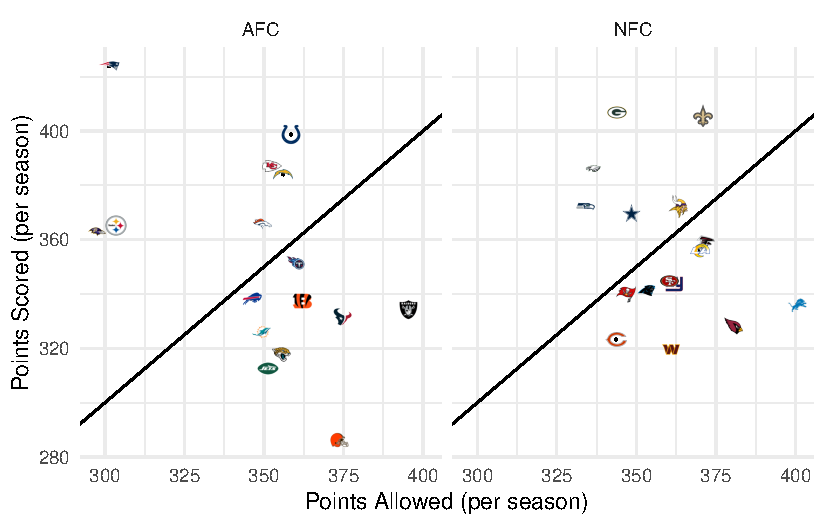
\includegraphics[keepaspectratio]{Final_Project_Team2_files/figure-pdf/fig-effeciency-scatter-plot-1.pdf}}

}

\end{figure}%

\subsection{AFC Effeciency Table}\label{afc-effeciency-table}

\begin{table}

\caption{\label{tbl-effeciency-scatter-plot-AFC}AFC Effeciency tables}

\centering{

\begin{longtabu} to \linewidth {>{\raggedright}X>{}c>{\centering}X>{\centering}X>{\centering}X}
\toprule
Team & image & Average Point Differential & Win Rate & Loss Rate\\
\midrule
NE & \includegraphics[width=0.17in, height=0.17in]{Logos/NE.png} & 122.5833 & 11.2500 & 4.8333\\
PIT & \includegraphics[width=0.17in, height=0.17in]{Logos/PIT.png} & 61.7500 & 10.0417 & 5.9167\\
IND & \includegraphics[width=0.17in, height=0.17in]{Logos/IND.png} & 40.1667 & 9.7500 & 6.2917\\
BAL & \includegraphics[width=0.17in, height=0.17in]{Logos/BAL.png} & 65.3750 & 9.4583 & 6.6250\\
KC & \includegraphics[width=0.17in, height=0.17in]{Logos/KC.png} & 34.5417 & 8.9583 & 7.1250\\
\addlinespace
DEN & \includegraphics[width=0.17in, height=0.17in]{Logos/DEN.png} & 16.2083 & 8.5417 & 7.5417\\
TEN & \includegraphics[width=0.17in, height=0.17in]{Logos/TEN.png} & -8.2917 & 8.4583 & 7.6250\\
LAC & \includegraphics[width=0.17in, height=0.17in]{Logos/LAC.png} & 28.0000 & 8.1667 & 7.9167\\
MIA & \includegraphics[width=0.17in, height=0.17in]{Logos/MIA.png} & -23.2917 & 7.7500 & 8.3333\\
BUF & \includegraphics[width=0.17in, height=0.17in]{Logos/BUF.png} & -8.0000 & 7.7083 & 8.3333\\
\addlinespace
CIN & \includegraphics[width=0.17in, height=0.17in]{Logos/CIN.png} & -24.5833 & 7.2917 & 8.5833\\
NYJ & \includegraphics[width=0.17in, height=0.17in]{Logos/NYJ.png} & -38.5417 & 7.0417 & 9.0417\\
HOU & \includegraphics[width=0.17in, height=0.17in]{Logos/HOU.png} & -43.1905 & 6.7619 & 9.2857\\
LV & \includegraphics[width=0.17in, height=0.17in]{Logos/LV.png} & -61.0417 & 6.5417 & 9.5417\\
JAX & \includegraphics[width=0.17in, height=0.17in]{Logos/JAX.png} & -37.8333 & 6.4167 & 9.6667\\
\addlinespace
CLE & \includegraphics[width=0.17in, height=0.17in]{Logos/CLE.png} & -87.4583 & 5.2917 & 10.7500\\
\bottomrule
\end{longtabu}

}

\end{table}%

\subsection{AFC Effeciency Table}\label{afc-effeciency-table-1}

\begin{table}

\caption{\label{tbl-effeciency-scatter-plot-NFC}NFC Effeciency tables}

\centering{

\begin{longtabu} to \linewidth {>{\raggedright}X>{}c>{\centering}X>{\centering}X>{\centering}X}
\toprule
Team & image & Average Point Differential & Win Rate & Loss Rate\\
\midrule
GB & \includegraphics[width=0.17in, height=0.17in]{Logos/NE.png} & 62.9167 & 9.9583 & 6.0417\\
PHI & \includegraphics[width=0.17in, height=0.17in]{Logos/PIT.png} & 49.7083 & 9.2500 & 6.7500\\
SEA & \includegraphics[width=0.17in, height=0.17in]{Logos/IND.png} & 38.2083 & 9.1250 & 6.9167\\
NO & \includegraphics[width=0.17in, height=0.17in]{Logos/BAL.png} & 34.7083 & 8.9167 & 7.1667\\
DAL & \includegraphics[width=0.17in, height=0.17in]{Logos/KC.png} & 21.4583 & 8.5833 & 7.5000\\
\addlinespace
MIN & \includegraphics[width=0.17in, height=0.17in]{Logos/DEN.png} & 9.2083 & 8.4583 & 7.5417\\
ATL & \includegraphics[width=0.17in, height=0.17in]{Logos/TEN.png} & -13.5417 & 7.7917 & 8.2500\\
LA & \includegraphics[width=0.17in, height=0.17in]{Logos/LAC.png} & -13.8333 & 7.6667 & 8.3750\\
NYG & \includegraphics[width=0.17in, height=0.17in]{Logos/MIA.png} & -18.1250 & 7.6667 & 8.3750\\
CAR & \includegraphics[width=0.17in, height=0.17in]{Logos/BUF.png} & -11.9167 & 7.5833 & 8.4583\\
\addlinespace
SF & \includegraphics[width=0.17in, height=0.17in]{Logos/CIN.png} & -15.7083 & 7.5417 & 8.5000\\
TB & \includegraphics[width=0.17in, height=0.17in]{Logos/NYJ.png} & -6.5417 & 7.5417 & 8.5417\\
CHI & \includegraphics[width=0.17in, height=0.17in]{Logos/HOU.png} & -20.3333 & 7.5000 & 8.5833\\
ARI & \includegraphics[width=0.17in, height=0.17in]{Logos/LV.png} & -52.2083 & 6.9167 & 9.0833\\
WAS & \includegraphics[width=0.17in, height=0.17in]{Logos/JAX.png} & -41.2500 & 6.8333 & 9.1667\\
\addlinespace
DET & \includegraphics[width=0.17in, height=0.17in]{Logos/CLE.png} & -64.5417 & 5.7917 & 10.2083\\
\bottomrule
\end{longtabu}

}

\end{table}%

\newpage{}

Code Appendix

\begin{Shaded}
\begin{Highlighting}[]
\CommentTok{\#|label: Packages}

\CommentTok{\#Tidyverse Coding Styling}
\FunctionTok{library}\NormalTok{(tidyverse)}
\FunctionTok{library}\NormalTok{(ggimage)}
\FunctionTok{library}\NormalTok{(kableExtra)}

\CommentTok{\#|label: Importing Data}

\NormalTok{NFL\_raw }\OtherTok{\textless{}{-}} \FunctionTok{read.csv}\NormalTok{(}\StringTok{"nfl{-}team{-}statistics (1).csv"}\NormalTok{)}

\CommentTok{\#|label: Adding East, West, North and South Conferences}
\NormalTok{NFC\_East\_data }\OtherTok{\textless{}{-}}\NormalTok{ NFL\_raw }\SpecialCharTok{\%\textgreater{}\%}
  \FunctionTok{filter}\NormalTok{(team }\SpecialCharTok{\%in\%} \FunctionTok{c}\NormalTok{(}\StringTok{"DAL"}\NormalTok{, }\StringTok{"NYG"}\NormalTok{, }\StringTok{"PHI"}\NormalTok{, }\StringTok{"WAS"}\NormalTok{))}\SpecialCharTok{\%\textgreater{}\%}
  \FunctionTok{mutate}\NormalTok{(}\AttributeTok{Conf =} \StringTok{\textquotesingle{}NFC\_East\textquotesingle{}}\NormalTok{)}

\NormalTok{NFC\_West\_data }\OtherTok{\textless{}{-}}\NormalTok{ NFL\_raw }\SpecialCharTok{\%\textgreater{}\%}
  \FunctionTok{filter}\NormalTok{(team }\SpecialCharTok{\%in\%} \FunctionTok{c}\NormalTok{(}\StringTok{"LA"}\NormalTok{, }\StringTok{"SEA"}\NormalTok{, }\StringTok{"SF"}\NormalTok{, }\StringTok{"ARI"}\NormalTok{))}\SpecialCharTok{\%\textgreater{}\%}
  \FunctionTok{mutate}\NormalTok{(}\AttributeTok{Conf =} \StringTok{\textquotesingle{}NFC\_West\textquotesingle{}}\NormalTok{)}

\NormalTok{NFC\_North\_data }\OtherTok{\textless{}{-}}\NormalTok{ NFL\_raw }\SpecialCharTok{\%\textgreater{}\%}
  \FunctionTok{filter}\NormalTok{(team }\SpecialCharTok{\%in\%} \FunctionTok{c}\NormalTok{(}\StringTok{"CHI"}\NormalTok{, }\StringTok{"GB"}\NormalTok{, }\StringTok{"DET"}\NormalTok{, }\StringTok{"MIN"}\NormalTok{))}\SpecialCharTok{\%\textgreater{}\%}
  \FunctionTok{mutate}\NormalTok{(}\AttributeTok{Conf =} \StringTok{\textquotesingle{}NFC\_North\textquotesingle{}}\NormalTok{)}

\NormalTok{NFC\_South\_data }\OtherTok{\textless{}{-}}\NormalTok{ NFL\_raw }\SpecialCharTok{\%\textgreater{}\%}
  \FunctionTok{filter}\NormalTok{(team }\SpecialCharTok{\%in\%} \FunctionTok{c}\NormalTok{(}\StringTok{"TB"}\NormalTok{, }\StringTok{"CAR"}\NormalTok{, }\StringTok{"ATL"}\NormalTok{, }\StringTok{"NO"}\NormalTok{))}\SpecialCharTok{\%\textgreater{}\%}
  \FunctionTok{mutate}\NormalTok{(}\AttributeTok{Conf =} \StringTok{\textquotesingle{}NFC\_South\textquotesingle{}}\NormalTok{)}

\NormalTok{AFC\_East\_data }\OtherTok{\textless{}{-}}\NormalTok{ NFL\_raw }\SpecialCharTok{\%\textgreater{}\%}
  \FunctionTok{filter}\NormalTok{(team }\SpecialCharTok{\%in\%} \FunctionTok{c}\NormalTok{(}\StringTok{"NE"}\NormalTok{, }\StringTok{"BUF"}\NormalTok{, }\StringTok{"MIA"}\NormalTok{, }\StringTok{"NYJ"}\NormalTok{))}\SpecialCharTok{\%\textgreater{}\%}
  \FunctionTok{mutate}\NormalTok{(}\AttributeTok{Conf =} \StringTok{\textquotesingle{}AFC\_East\textquotesingle{}}\NormalTok{)}

\NormalTok{AFC\_West\_data }\OtherTok{\textless{}{-}}\NormalTok{ NFL\_raw }\SpecialCharTok{\%\textgreater{}\%}
  \FunctionTok{filter}\NormalTok{(team }\SpecialCharTok{\%in\%} \FunctionTok{c}\NormalTok{(}\StringTok{"DEN"}\NormalTok{, }\StringTok{"LAC"}\NormalTok{, }\StringTok{"KC"}\NormalTok{, }\StringTok{"LV"}\NormalTok{))}\SpecialCharTok{\%\textgreater{}\%}
  \FunctionTok{mutate}\NormalTok{(}\AttributeTok{Conf =} \StringTok{\textquotesingle{}AFC\_West\textquotesingle{}}\NormalTok{)}

\NormalTok{AFC\_North\_data }\OtherTok{\textless{}{-}}\NormalTok{ NFL\_raw }\SpecialCharTok{\%\textgreater{}\%}
  \FunctionTok{filter}\NormalTok{(team }\SpecialCharTok{\%in\%} \FunctionTok{c}\NormalTok{(}\StringTok{"BAL"}\NormalTok{, }\StringTok{"PIT"}\NormalTok{, }\StringTok{"CIN"}\NormalTok{, }\StringTok{"CLE"}\NormalTok{))}\SpecialCharTok{\%\textgreater{}\%}
  \FunctionTok{mutate}\NormalTok{(}\AttributeTok{Conf =} \StringTok{\textquotesingle{}AFC\_North\textquotesingle{}}\NormalTok{)}

\NormalTok{AFC\_South\_data }\OtherTok{\textless{}{-}}\NormalTok{ NFL\_raw }\SpecialCharTok{\%\textgreater{}\%}
  \FunctionTok{filter}\NormalTok{(team }\SpecialCharTok{\%in\%} \FunctionTok{c}\NormalTok{(}\StringTok{"JAX"}\NormalTok{, }\StringTok{"IND"}\NormalTok{, }\StringTok{"HOU"}\NormalTok{, }\StringTok{"TEN"}\NormalTok{))}\SpecialCharTok{\%\textgreater{}\%}
  \FunctionTok{mutate}\NormalTok{(}\AttributeTok{Conf =} \StringTok{\textquotesingle{}AFC\_South\textquotesingle{}}\NormalTok{)}

\NormalTok{NFL\_Clean }\OtherTok{\textless{}{-}} \FunctionTok{bind\_rows}\NormalTok{(NFC\_East\_data, NFC\_North\_data, NFC\_South\_data, NFC\_West\_data, AFC\_East\_data, AFC\_South\_data, AFC\_North\_data, AFC\_West\_data) }\SpecialCharTok{\%\textgreater{}\%}
  \FunctionTok{arrange}\NormalTok{(season, team)}\SpecialCharTok{\%\textgreater{}\%}
    \FunctionTok{separate\_wider\_delim}\NormalTok{(}
    \AttributeTok{cols =} \StringTok{\textquotesingle{}Conf\textquotesingle{}}\NormalTok{,}
    \AttributeTok{delim =} \StringTok{\textquotesingle{}\_\textquotesingle{}}\NormalTok{,}
    \AttributeTok{names =} \FunctionTok{c}\NormalTok{(}\StringTok{\textquotesingle{}Conf\textquotesingle{}}\NormalTok{, }\StringTok{\textquotesingle{}Div\textquotesingle{}}\NormalTok{)}
\NormalTok{  )}

\NormalTok{NFL\_Clean\_3 }\OtherTok{\textless{}{-}}\NormalTok{ NFL\_Clean }\SpecialCharTok{\%\textgreater{}\%}
  \FunctionTok{select}\NormalTok{(team, Conf, score\_differential, points\_scored,}
\NormalTok{         points\_allowed, wins, losses) }\SpecialCharTok{\%\textgreater{}\%}
  \FunctionTok{group\_by}\NormalTok{(team, Conf) }\SpecialCharTok{\%\textgreater{}\%}
  \FunctionTok{summarise}\NormalTok{(}
    \AttributeTok{points\_scored =} \FunctionTok{mean}\NormalTok{(points\_scored),}
    \AttributeTok{points\_allowed =} \FunctionTok{mean}\NormalTok{(points\_allowed),}
    \AttributeTok{wins =} \FunctionTok{mean}\NormalTok{(wins),}
    \AttributeTok{losses =} \FunctionTok{mean}\NormalTok{(losses),}
    \AttributeTok{point\_differential =} \FunctionTok{mean}\NormalTok{(score\_differential),}
    \AttributeTok{.groups =} \StringTok{"drop"}
\NormalTok{  )}
\NormalTok{NFL\_Clean\_3}\SpecialCharTok{$}\NormalTok{logo }\OtherTok{\textless{}{-}} \FunctionTok{paste0}\NormalTok{(}\StringTok{"Logos/"}\NormalTok{, NFL\_Clean\_3}\SpecialCharTok{$}\NormalTok{team, }\StringTok{".png"}\NormalTok{)}

\FunctionTok{ggplot}\NormalTok{(NFL\_Clean\_3) }\SpecialCharTok{+}
  \FunctionTok{aes}\NormalTok{(}\AttributeTok{x =}\NormalTok{ points\_allowed, }\AttributeTok{y =}\NormalTok{ points\_scored) }\SpecialCharTok{+}
  \FunctionTok{geom\_point}\NormalTok{(}\AttributeTok{size =} \FloatTok{0.1}\NormalTok{) }\SpecialCharTok{+}
  \FunctionTok{geom\_image}\NormalTok{(}\FunctionTok{aes}\NormalTok{(}\AttributeTok{image =}\NormalTok{ logo)) }\SpecialCharTok{+}
  \FunctionTok{labs}\NormalTok{(}
    \AttributeTok{x =} \StringTok{"Points Allowed (per season)"}\NormalTok{,}
    \AttributeTok{y =} \StringTok{"Points Scored (per season)"}
\NormalTok{  ) }\SpecialCharTok{+}
  \FunctionTok{geom\_abline}\NormalTok{(}\AttributeTok{slope =} \DecValTok{1}\NormalTok{, }\AttributeTok{intercept =} \DecValTok{0}\NormalTok{) }\SpecialCharTok{+}
  \FunctionTok{theme\_minimal}\NormalTok{() }\SpecialCharTok{+}
  \FunctionTok{facet\_wrap}\NormalTok{(}\FunctionTok{vars}\NormalTok{(Conf))}

\NormalTok{AFC\_table }\OtherTok{\textless{}{-}}\NormalTok{ NFL\_Clean\_3}\SpecialCharTok{\%\textgreater{}\%}
  \FunctionTok{filter}\NormalTok{(Conf }\SpecialCharTok{==} \StringTok{\textquotesingle{}AFC\textquotesingle{}}\NormalTok{)}\SpecialCharTok{\%\textgreater{}\%}
  \FunctionTok{select}\NormalTok{(team, point\_differential, wins, losses, logo)}\SpecialCharTok{\%\textgreater{}\%}
  \FunctionTok{mutate}\NormalTok{(}
    \AttributeTok{point\_differential =} \FunctionTok{round}\NormalTok{(point\_differential, }\AttributeTok{digits =} \DecValTok{4}\NormalTok{),}
    \AttributeTok{wins =} \FunctionTok{round}\NormalTok{(wins, }\AttributeTok{digits =} \DecValTok{4}\NormalTok{),}
    \AttributeTok{losses =} \FunctionTok{round}\NormalTok{(losses, }\AttributeTok{digits =} \DecValTok{4}\NormalTok{),}
    \AttributeTok{image =} \StringTok{""}
\NormalTok{  )}\SpecialCharTok{\%\textgreater{}\%}
  \FunctionTok{arrange}\NormalTok{(}\FunctionTok{desc}\NormalTok{(wins)) }\SpecialCharTok{\%\textgreater{}\%}
  \FunctionTok{rename}\NormalTok{(}
    \AttributeTok{Team =}\NormalTok{ team,}
    \StringTok{\textasciigrave{}}\AttributeTok{Average Point Differential}\StringTok{\textasciigrave{}} \OtherTok{=}\NormalTok{ point\_differential,}
    \StringTok{\textasciigrave{}}\AttributeTok{Win Rate}\StringTok{\textasciigrave{}} \OtherTok{=}\NormalTok{ wins,}
    \StringTok{\textasciigrave{}}\AttributeTok{Loss Rate}\StringTok{\textasciigrave{}} \OtherTok{=}\NormalTok{ losses}
\NormalTok{  )}

\NormalTok{AFC\_table }\SpecialCharTok{\%\textgreater{}\%}
  \FunctionTok{select}\NormalTok{(Team, image, }\StringTok{\textasciigrave{}}\AttributeTok{Average Point Differential}\StringTok{\textasciigrave{}}\NormalTok{, }\StringTok{\textasciigrave{}}\AttributeTok{Win Rate}\StringTok{\textasciigrave{}}\NormalTok{, }\StringTok{\textasciigrave{}}\AttributeTok{Loss Rate}\StringTok{\textasciigrave{}}\NormalTok{) }\SpecialCharTok{\%\textgreater{}\%}
  \FunctionTok{kable}\NormalTok{(}\AttributeTok{booktabs =} \ConstantTok{TRUE}\NormalTok{,}
        \AttributeTok{align =} \FunctionTok{c}\NormalTok{(}\StringTok{"l"}\NormalTok{, }\FunctionTok{rep}\NormalTok{(}\StringTok{"c"}\NormalTok{, }\DecValTok{10}\NormalTok{)))}\SpecialCharTok{\%\textgreater{}\%}
  \FunctionTok{kable\_styling}\NormalTok{()}\SpecialCharTok{\%\textgreater{}\%}
  \FunctionTok{kable\_paper}\NormalTok{(}\AttributeTok{full\_width =}\NormalTok{ T)}\SpecialCharTok{\%\textgreater{}\%}
  \FunctionTok{column\_spec}\NormalTok{(}\DecValTok{2}\NormalTok{, }\AttributeTok{image =} \FunctionTok{spec\_image}\NormalTok{(}\AttributeTok{path =}\NormalTok{ AFC\_table}\SpecialCharTok{$}\NormalTok{logo, }\DecValTok{50}\NormalTok{, }\DecValTok{50}\NormalTok{))}

\NormalTok{NFC\_table }\OtherTok{\textless{}{-}}\NormalTok{ NFL\_Clean\_3}\SpecialCharTok{\%\textgreater{}\%}
  \FunctionTok{filter}\NormalTok{(Conf }\SpecialCharTok{==} \StringTok{\textquotesingle{}NFC\textquotesingle{}}\NormalTok{)}\SpecialCharTok{\%\textgreater{}\%}
  \FunctionTok{select}\NormalTok{(team, point\_differential, wins, losses, logo)}\SpecialCharTok{\%\textgreater{}\%}
  \FunctionTok{mutate}\NormalTok{(}
    \AttributeTok{point\_differential =} \FunctionTok{round}\NormalTok{(point\_differential, }\AttributeTok{digits =} \DecValTok{4}\NormalTok{),}
    \AttributeTok{wins =} \FunctionTok{round}\NormalTok{(wins, }\AttributeTok{digits =} \DecValTok{4}\NormalTok{),}
    \AttributeTok{losses =} \FunctionTok{round}\NormalTok{(losses, }\AttributeTok{digits =} \DecValTok{4}\NormalTok{),}
    \AttributeTok{image =} \StringTok{""}
\NormalTok{  )}\SpecialCharTok{\%\textgreater{}\%}
  \FunctionTok{arrange}\NormalTok{(}\FunctionTok{desc}\NormalTok{(wins)) }\SpecialCharTok{\%\textgreater{}\%}
  \FunctionTok{rename}\NormalTok{(}
    \AttributeTok{Team =}\NormalTok{ team,}
    \StringTok{\textasciigrave{}}\AttributeTok{Average Point Differential}\StringTok{\textasciigrave{}} \OtherTok{=}\NormalTok{ point\_differential,}
    \StringTok{\textasciigrave{}}\AttributeTok{Win Rate}\StringTok{\textasciigrave{}} \OtherTok{=}\NormalTok{ wins,}
    \StringTok{\textasciigrave{}}\AttributeTok{Loss Rate}\StringTok{\textasciigrave{}} \OtherTok{=}\NormalTok{ losses}
\NormalTok{  )}

\NormalTok{NFC\_table }\SpecialCharTok{\%\textgreater{}\%}
  \FunctionTok{select}\NormalTok{(Team, image, }\StringTok{\textasciigrave{}}\AttributeTok{Average Point Differential}\StringTok{\textasciigrave{}}\NormalTok{, }\StringTok{\textasciigrave{}}\AttributeTok{Win Rate}\StringTok{\textasciigrave{}}\NormalTok{, }\StringTok{\textasciigrave{}}\AttributeTok{Loss Rate}\StringTok{\textasciigrave{}}\NormalTok{) }\SpecialCharTok{\%\textgreater{}\%}
  \FunctionTok{kable}\NormalTok{(}\AttributeTok{booktabs =} \ConstantTok{TRUE}\NormalTok{,}
        \AttributeTok{align =} \FunctionTok{c}\NormalTok{(}\StringTok{"l"}\NormalTok{, }\FunctionTok{rep}\NormalTok{(}\StringTok{"c"}\NormalTok{, }\DecValTok{10}\NormalTok{)))}\SpecialCharTok{\%\textgreater{}\%}
  \FunctionTok{kable\_styling}\NormalTok{()}\SpecialCharTok{\%\textgreater{}\%}
  \FunctionTok{kable\_paper}\NormalTok{(}\AttributeTok{full\_width =}\NormalTok{ T)}\SpecialCharTok{\%\textgreater{}\%}
  \FunctionTok{column\_spec}\NormalTok{(}\DecValTok{2}\NormalTok{, }\AttributeTok{image =} \FunctionTok{spec\_image}\NormalTok{(}\AttributeTok{path =}\NormalTok{ AFC\_table}\SpecialCharTok{$}\NormalTok{logo, }\DecValTok{50}\NormalTok{, }\DecValTok{50}\NormalTok{))}
\end{Highlighting}
\end{Shaded}





\end{document}
